\section*{Recurrent Neural Networks}
\subsection*{Simple RNNs}
Given a sequence of observations $\mathbf x^1,...,\mathbf x^s$, not iid\\
Discrete time evolution of hidden state space sequence: \\$\mathbf h^t=F(\mathbf h^{t-1},\mathbf x^t;\pmb\theta) \Rightarrow$ Markov property and time-invariant\\
$\mathbf h^{t}=F(\mathbf h^{t-1},\mathbf x^{t};\pmb\theta)=\sigma\circ\bar F(\mathbf h^{t-1},\mathbf x^{t};\pmb\theta), \quad \bar F(\mathbf h, \mathbf x; \pmb\theta)=\mathbf{Wh+Ux+b}$\\
Optionally produce outputs: $\mathbf y^t=H(\mathbf h^t;\pmb\theta), \quad H(\mathbf h, \pmb\theta):=\sigma(\mathbf{Vh+c})$
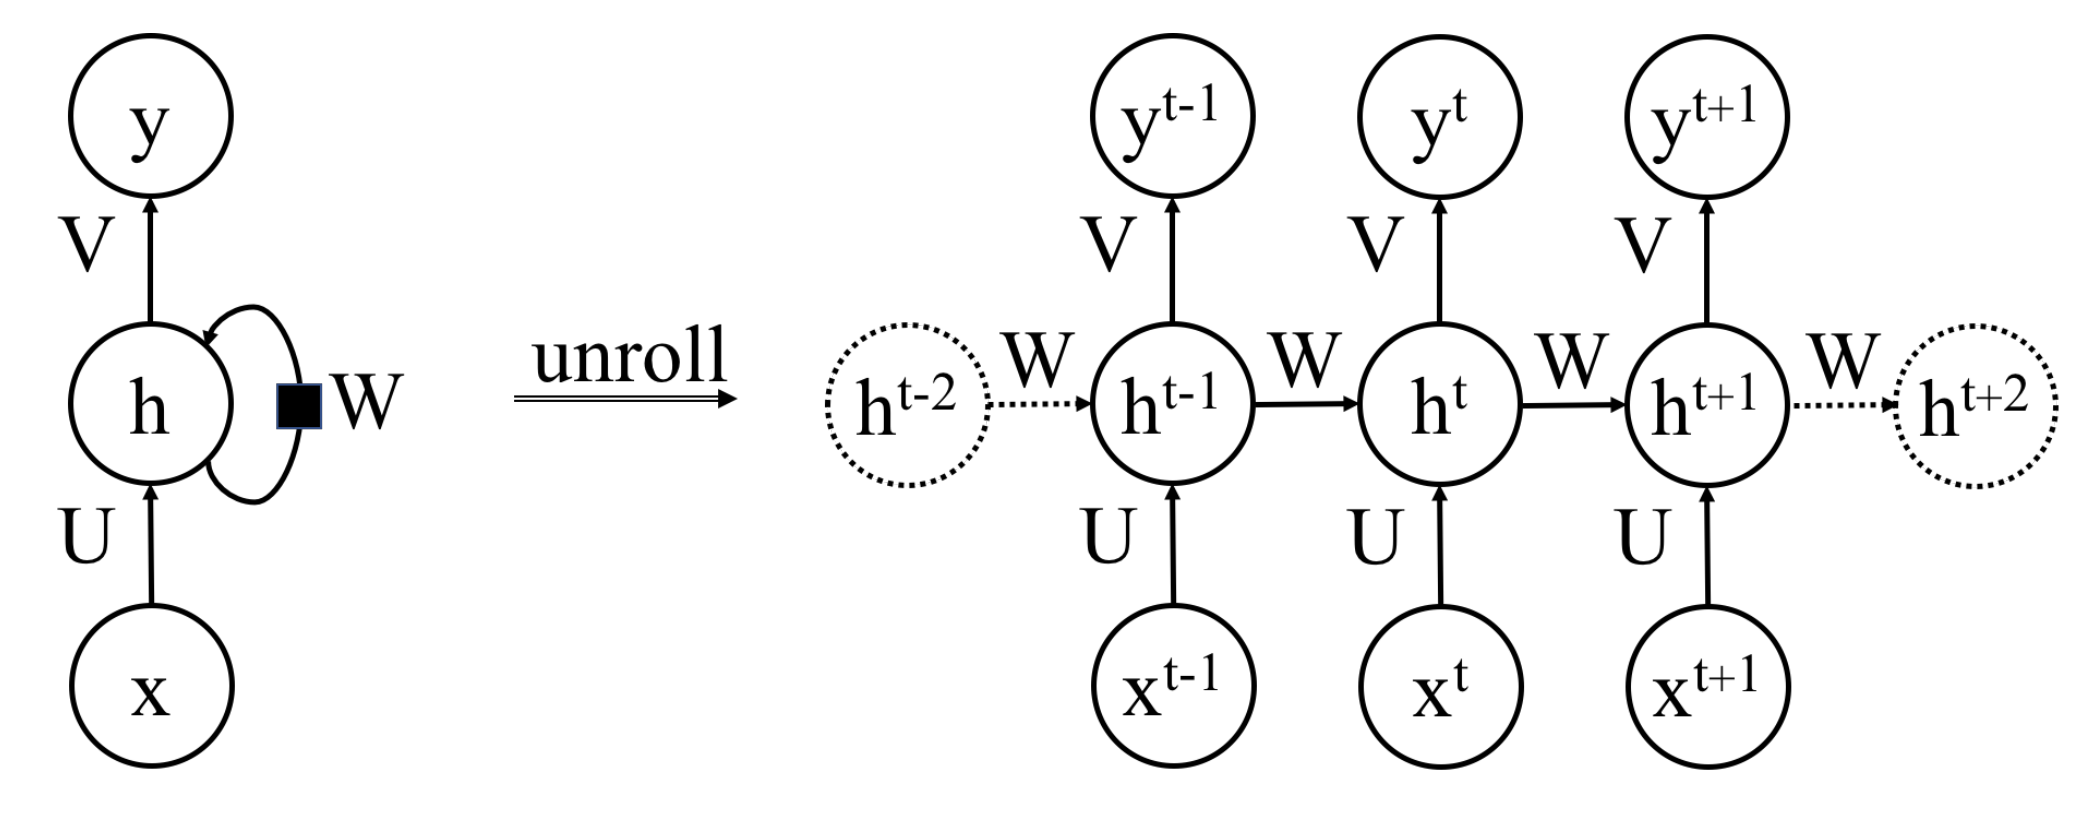
\includegraphics[width=0.9\linewidth]{rnn_unrolled.png}
\\Hidden state can be thought of as a noisy memory, compresses relevant aspects of sequence: $(\mathbf x^1,...,\mathbf x^{t-1})\mapsto \mathbf h^t$ (conceptually)\\
 For any fixed length $s$, the unrolled recurrent net corresponds to a feedforward net with $s$ hidden layers. Difference to MLP: sharing of parameters and inputs processed sequentially..\\
\textbf{Backpropagation (through time :P)}: sum over time steps\\
With $\dot\sigma_i^t:=\sigma'(\bar F_i(h^{t-1},x^t))$:\\
$\frac{\partial\mathcal R}{\partial w_{ij}}=\sum_{t=1}^s\frac{\partial\mathcal R}{\partial h_i^t}\cdot\frac{\partial h_i^t}{\partial w_{ij}}=\sum_{t=1}^s\frac{\partial\mathcal R}{\partial h_i^t}\cdot\dot\sigma_i^t\cdot h_j^{t-1}$\\
$\frac{\partial\mathcal R}{\partial u_{ik}}=\sum_{t=1}^s\frac{\partial\mathcal R}{\partial h_i^t}\cdot\frac{\partial h_i^t}{\partial u_{ik}}=\sum_{t=1}^s\frac{\partial\mathcal R}{\partial h_i^t}\cdot\dot\sigma_i^t\cdot x_k^{t}$\\
Example with setting: $y_{1:T}$ ground-truth outputs and $\hat y_{1:T}$ predictions, $a_t=F(x_t,h_{t-1},y_{t-1};\theta)$, $h_t=\sigma(a_t)$, $\hat y_t=G(h_t,\phi)$, $L_t=H(y_t,\hat y_t)$, $L=\sum_{t=1}^TL_t$. Derivative of $L$ wrt $\theta$:\\
$\frac{\partial L}{\partial \theta}=\sum_{t=1}^T\frac{\partial L_t}{\partial \hat y_t}\frac{\partial \hat y_t}{\partial h_t}\sum_{i=0}^t(\prod_{j=t}^{i+1}\frac{\partial h_j}{\partial a_j}\frac{\partial a_j}{\partial h_{j-1}})\frac{\partial h_i}{\partial a_i}\frac{\partial a_i}{\partial\theta}$\\
\textbf{Exploding/Vanishing gradients}: let  output in last step $\mathbf y=\mathbf y^s$\\
Then $\nabla_{\mathbf x^t}\mathcal R=[\prod_{r=t+1}^s\mathbf W^T\mathbf{S}(\mathbf h^r)]\cdot\mathbf J_H\cdot\nabla_\mathbf y\mathcal R, \quad \mathbf{S}(\mathbf h^r)=\text{diag}(\dot\sigma_1^r,...,\dot\sigma_n^r)$\\
Take spectral norm, and use $||\mathbf{AB}||_2\leq||\mathbf A||_2\cdot||\mathbf B||_2$. If $\sigma_{\max}(\mathbf W)<1$:\\ $||\nabla_{\mathbf x^t}\mathcal R||\leq\sigma_{\max}(\mathbf W)^{s-t}\cdot||\mathbf \mathbf J_H\cdot\nabla_\mathbf y\mathcal R||\overset{(s-t)\rightarrow\infty}{\rightarrow}0$\\
Conversely may explode if $\sigma_{\max}(\mathbf W)>1$\\
\textbf{Bi-directional network}: reverse order $\mathbf g^t=G(\mathbf x^t,\mathbf g^{t+1};\pmb\theta)$\\
Interweave the two hidden state sequences\\
\textbf{Deep recurrent network:} hierarchical hidden states of $l$ layers\\
$\mathbf h^{t,1}=F(\mathbf h^{t-1,1},\mathbf x^t;\pmb\theta)$\\
$\mathbf h^{t,l}=F(\mathbf h^{t-1,l},\mathbf h^{t,l-1};\pmb\theta), \quad l=2,...,L$
\subsection*{Memory Units}
\textit{Addressing the problem of vanishing/exploding gradients}\\
Gated units to learn long-term dependencies\\
Difficult to understand what units learn, resource-hungry and slow in learning\\
\textbf{LSTM}\\
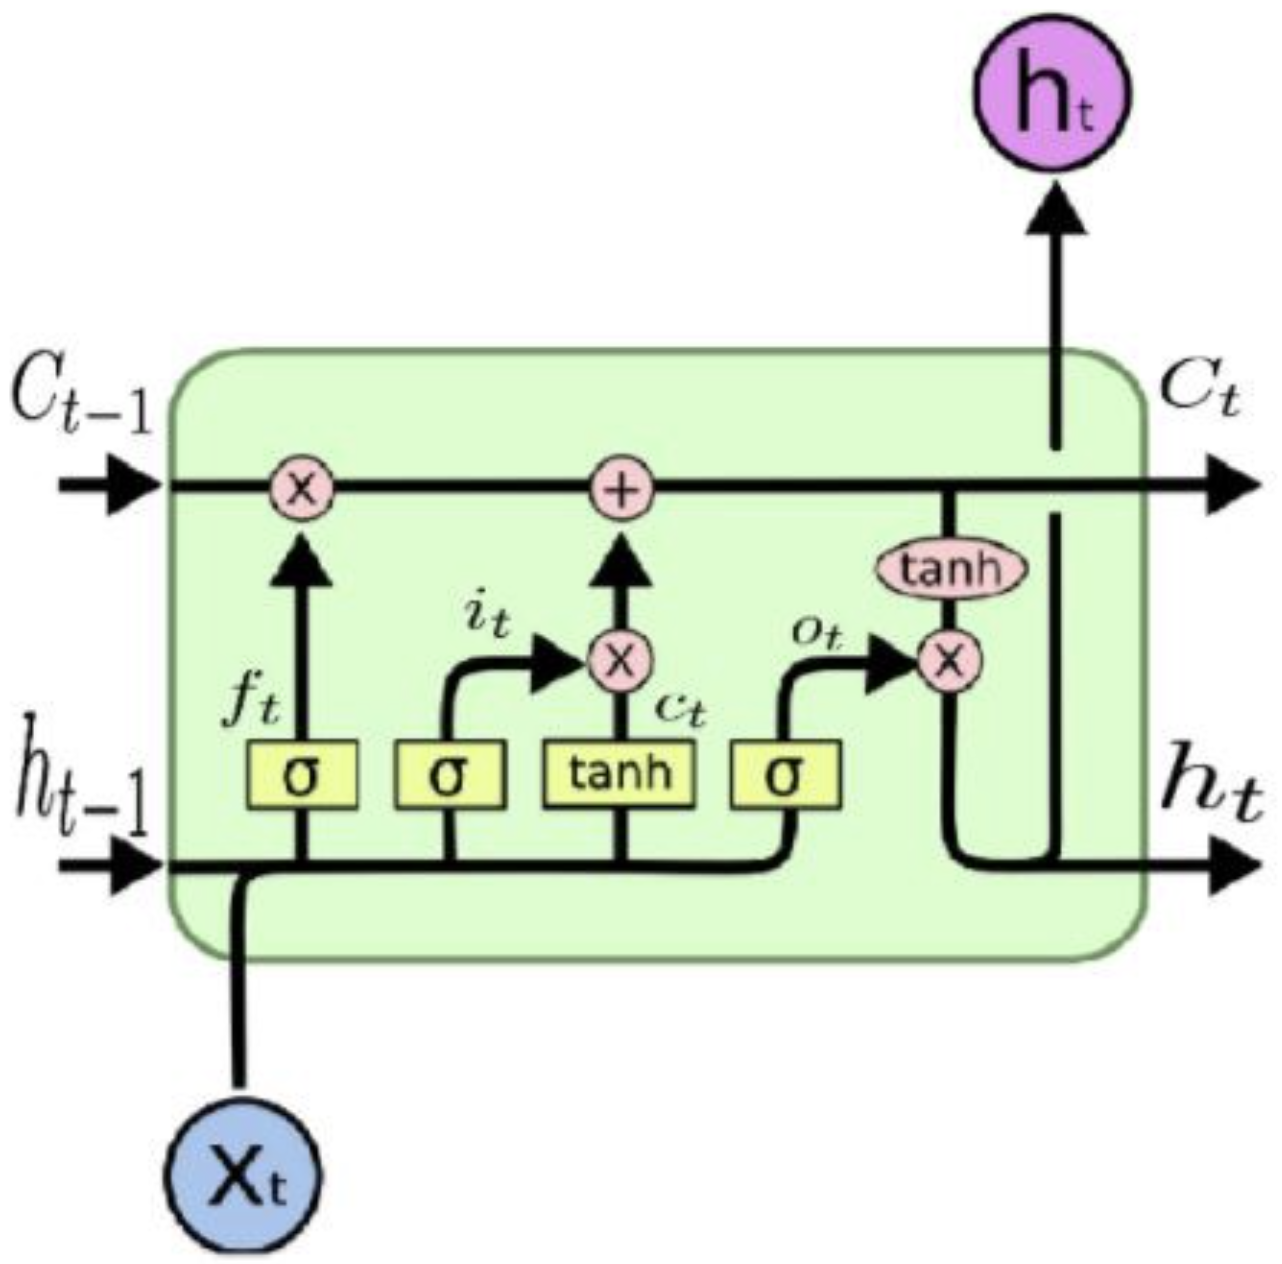
\includegraphics[scale=0.17]{lstm_cell.png}
\\Content $C$ has similar effect as ResNet for vanishing gradients\\
Forget gate: $f_t=\sigma(W_f\cdot[h_{t-1},x_t]+b_f)$\\
Input to memory: \\ $i_t=\sigma(W_i\cdot[h_{t-1},x_t]+b_i), \quad $
$\tilde C_t=\tanh (W_C\cdot[h_{t-1},x_t]+b_C)$\\
Updating memory: $C_t=f_t*C_{t-1}+i_t*\tilde C_t$\\
Output gate:\\
$o_t=\sigma(W_o[h_{t-1},x_t]+b_o), \quad h_t=o_t*\tanh (C_t)$\\
Gates: input gate, output gate and forget gate\\
\textbf{Gated Recurrent Unit (GRU)}\\
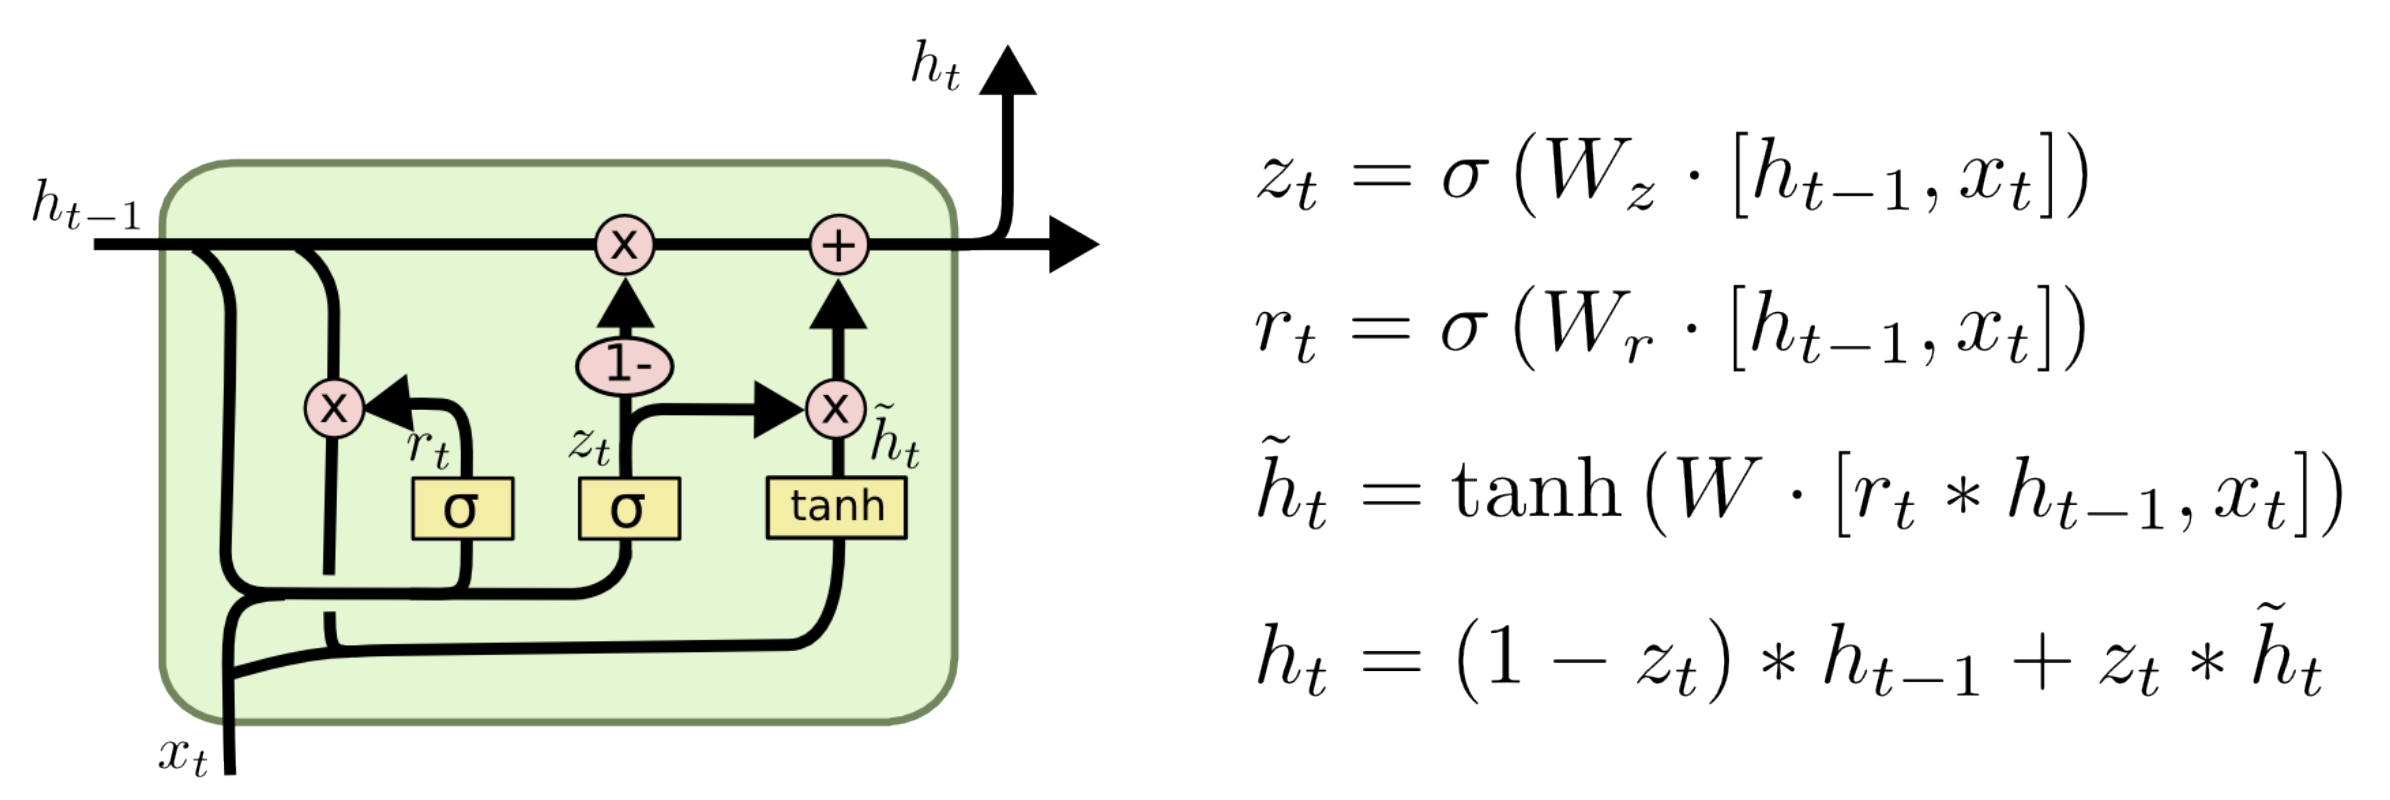
\includegraphics[scale=0.17]{gru.png}\\
Gates: update gate and reset gate \\
Here $h$ is both state and content, computed as a convex combination of old and new information
\subsection*{Learning sequences - Seq2Seq}
Goal: learn $p(\mathbf y^{1:T}|\mathbf x^{1:T})\approx \prod_{t=1}^Tp(\mathbf y^t|\mathbf x^{1:t},\mathbf y^{1:t-1})$\\
Naive implementation: $p(\mathbf y^t)$ depends on $\mathbf y^{1:t-1}$ only through $\mathbf h^t$\\
$\Rightarrow$ remedy by feeding back previous outputs!\\
\textbf{Teacher forcing:} When training, compute loss on predicted output but feed back in correct output. During prediction feed back predicted outputs. Improves learning BUT gives exposure bias\\
\textbf{Encoder-Decoder model}: \\
Encoder: $(\mathbf x^1,...,\mathbf x^T)\mapsto \mathbf z, \quad \mathbf z=\mathbf h^T$ (RNN)\\
Decoder $\mathbf z\mapsto (\mathbf y^1,...,\mathbf y^S)$ (RNN with output feedback)\\
Can also be used for image captioning with CNN encoder